\documentclass[9pt]{beamer}

\usepackage{préambule}
\usepackage{tcolorbox}

\setbeamersize{
	text margin left=0.5cm,
	text margin right=0.5cm
}

\begin{document}

\begin{frame}
	\begin{multicols}{3}
		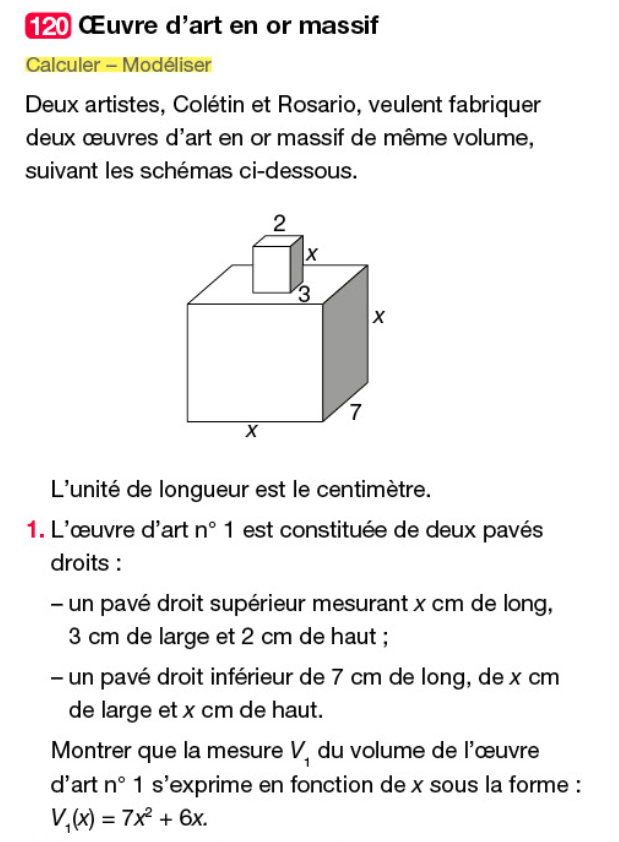
\includegraphics[width=\linewidth]{Images/Exercice 120 page 77 - question 1.png}

		\columnbreak

		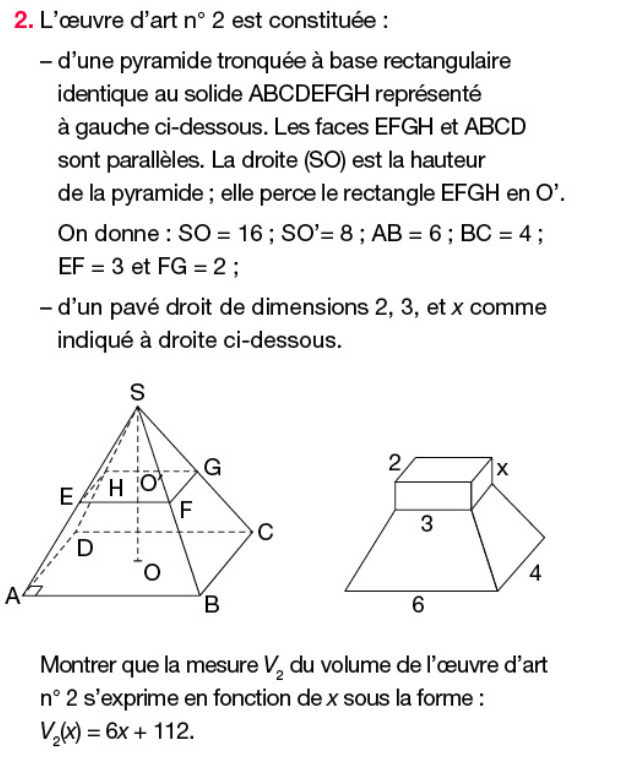
\includegraphics[width=\linewidth]{Images/Exercice 120 page 77 - question 2.png}

		\columnbreak

		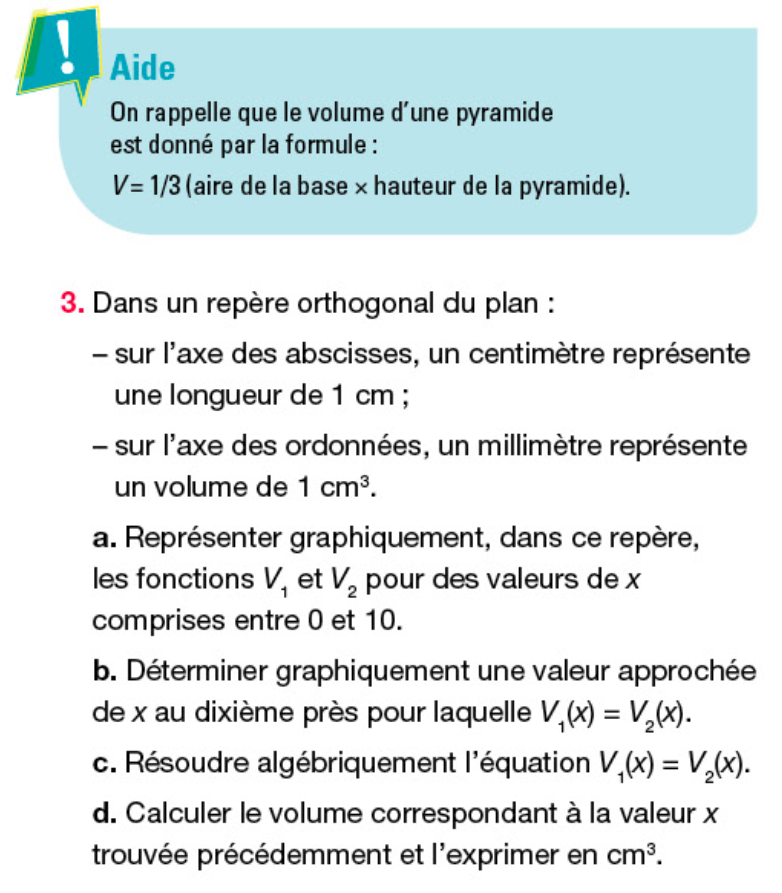
\includegraphics[width=\linewidth]{Images/Exercice 120 page 77 - question 3.png}
	\end{multicols}
\end{frame}

\begin{frame}
	\scriptsize

	\begin{multicols}{3}
		\underline{Exercice 120 page 77} \medskip

		Deux artistes, Colétin et Rosario, veulent fabriquer deux œuvres d'art en or massif de même volume, suivant les schémas ci-dessous.

		\begin{center}
			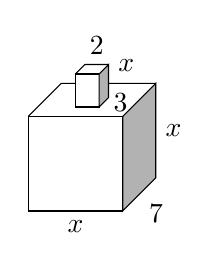
\begin{tikzpicture}[scale=0.6]
				\draw (0,0) -- node[below] {$x$} (2,0) -- (2,2) -- (0,2) -- cycle;
				\draw[fill=gray!60] (2,0) -- node[midway,below right] {$7$} ++(0.7,0.7) -- node[midway,right] {$x$} ++(0,2) -- ++(-0.7,-0.7) -- cycle;
				\draw (0,2) -- ++(0.7,0.7) -- ++(2,0);

				\draw[fill=white] (1,2.2) -- ++(0.5,0) -- ++(0,0.7) -- ++(-0.5,0) -- cycle;
				\draw[fill=gray!60] (1.5,2.2) -- node[midway,right] {3} ++(0.2,0.2) -- node[midway,above right] {$x$} ++(0,0.7) -- ++(-0.2,-0.2) -- cycle;
				\draw (1,2.9) -- ++(0.2,0.2) -- node[above] {2} ++(0.5,0);
			\end{tikzpicture}
		\end{center}
		L'unité de longueur est le centimètre. \medskip

		\hspace{-1em}{\color{blue}1.} L'œuvre d'art n°1 est constituée de deux pavés droits : \medskip

		- un pavé droit supérieur mesurant $x$ cm de long, $3$ cm de large et $2$ cm de haut ; \medskip

		- un pavé droit inférieur de $7$ cm de long, $x$ cm de large et $x$ cm de haut. \medskip

		Montrer que la mesure $V₁$ du volume de l'œuvre d'art n°1 s'exprime en fonction de $x$ sous la forme :

		$V₁(x) = 7x² + 6x$.

		\columnbreak

		\hspace{-1em}{\color{blue}2.} L'œuvre d'art n°2 est constituée : \smallskip

		- d'une pyramide tronquée à base rectangulaire identique au solide ABCDEFGH représenté à gauche ci-dessous. Les faces EFGH et ABCD sont parallèles. La droite (SO) est la hauteur de la pyramide ; elle perce le rectangle EFGH en O'. \smallskip

		On donne : SO = 16 ; SO' = 8 ;

		AB = 6 ; BC = 4 ; EF = 3

		et FG = 2 ; \smallskip

		- d'un pavé droit de dimensions 2, 3 et $x$ comme indiqué à droite ci-dessous.

		\begin{center}
			\tiny
			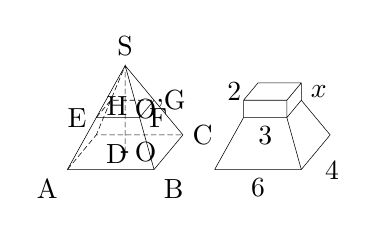
\begin{tikzpicture}[scale=1.1]
				\coordinate (A) at (0,0);
				\coordinate (B) at (1,0);
				\coordinate (C) at (4/3,0.4);
				\coordinate (D) at (1/3,0.4);
				\coordinate (E) at (1/3,0.6);
				\coordinate (F) at (5/6,0.6);
				\coordinate (G) at (1,0.8);
				\coordinate (H) at (0.5,0.8);
				\coordinate (S) at (2/3,1.2);
				\coordinate (O) at (2/3,0.2);
				\coordinate (O') at (2/3,0.7);

				\foreach \p/\pos in {
						A/below left,
						B/below right,
						C/right,
						D/below right,
						E/left,
						F/right,
						G/right,
						S/above,
						O/right,
						O'/right} {
						\node[\pos] at (\p) {\p};
					}
				\node[xshift=0.08cm,yshift=-0.08cm] at (H) {H};
				\node at (O) {-};
				\draw[very thin] (A) -- (B) -- (C) -- (S) -- (A)
				(E) -- (F) -- (G)
				(S) -- (B);
				\draw[very thin,dash pattern={on 2pt off 1pt}] (A) -- (D) -- (C)
				(O) -- (S) -- (D)
				(E) -- (H) -- (G);

				\draw[very thin] (1.7,0)
				-- node[midway,below] {6} ++(1,0)
				-- node[midway,below right] {4} ++(1/3,0.4)
				-- ++(-1/3,0.4)
				-- node[midway,right] {$x$} ++(0,0.2)
				-- ++(-0.5,0)
				-- node[midway,left] {2} ++(-1/6,-0.2)
				-- ++(0,-0.2)
				-- node[midway,below] {3} ++(0.5,0)
				-- ++(1/6,-0.6)
				(1.7,0)
				-- ++(1/3,0.6)
				++(4/6,0.2)
				-- ++(-1/6,-0.2)
				-- ++(0,0.2)
				-- ++(-0.5,0)
				++(0.5,0)
				-- ++(1/6,0.2);
			\end{tikzpicture}
		\end{center}

		Montrer que la mesure $V₂$ du volume de l'œuvre d'art n°2 s'exprime en fonction de $x$ sous la forme :

		$V₂(x) = 6x + 112$.

		\columnbreak

		\begin{tcolorbox}
			{\small Aide}
			\tiny

			On rappelle que le volume d'une pyramide est donné par la formule :

			$V = 1/3$(aire de la base $×$ hauteur de la pyramide).
		\end{tcolorbox}

		\hspace{-1em}{\color{blue}3.} Dans un repère orthogonal du plan : \smallskip

		- sur l'axe des abscisses, un centimètre représente une longueur de 1 cm ; \smallskip

		- sur l'axe des ordonnées, un millimètre représente un volume de 1 cm³. \smallskip

		\textbf{a.} Représenter graphiquement, dans ce repère, les fonctions $V₁$ et $V₂$ pour des valeurs de $x$ comprises entre 0 et 10.  \smallskip

		\textbf{b.} Déterminer graphiquement une valeur approchée de $x$ au dixième près pour laquelle $V₁(x) = V₂(x)$.  \smallskip

		\textbf{c.} Résoudre algébriquement l'équation $V₁(x) = V₂(x)$. \smallskip

		\textbf{d.} Calculer le volume correspondant à la valeur $x$ trouvée précédemment, et l'exprimer en cm³.  \smallskip
	\end{multicols}
\end{frame}

\end{document}